\section{Dados do sensor laser}
Essa Seção explica o formato dos dados brutos do sensor LiDAR, e como eles 
são processados e transformados nos dados utilizados pelo modelo de medida 
descrito na Seção \ref{sec:slam-measurement} (\nameref{sec:slam-measurement}).

\subsection{Dados brutos}
Os dados brutos do sensor LiDAR utilizado, consistem numa sequência de 
distâncias $\{r^0, r^1, \dots, r^N\}$. Esses valores são gerados pela reflexão de feixes de laser, emitidos pelo sensor, nas superfícies 
presentes no ambiente. Os feixes são disparados de maneira sequencial no 
sentido anti-horário a partir do eixo $x$ do sistema de coordenadas do sensor. 
Além disso, o sensor também fornece as posições angulares $\theta_0$ 
do primeiro e $\theta_N$ do último feixe, e o incremento na posição angular $\Delta \theta$ entre o feixe $k+1$ e o feixe $k$.

A Figura \ref{fig:sensor-raw-data} apresenta os dados brutos obtidos em uma 
leitura feita no ambiente mostrado na Figura \ref{fig:environment}.

\begin{figure}[h]
  \centering
  \begin{subfigure}{0.6\textwidth}
    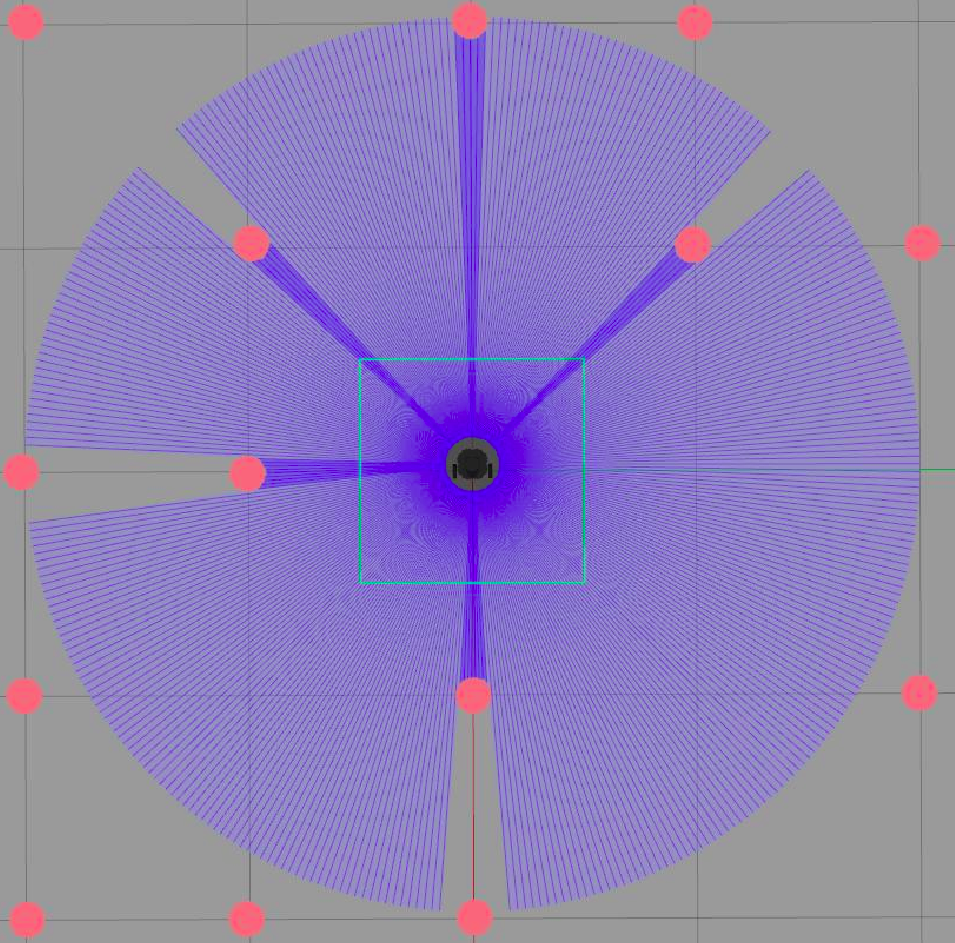
\includegraphics[width=\textwidth, angle=90]{figs/sensor-simulation-view.png}
    \caption{Representação dos feixes laser (em azul) emitidos pelo sensor LiDAR com 
    alcance máximo de 2 metros. Os círculos em rosa representam as landmarks.}
    \label{fig:laser-beams-visualization}
  \end{subfigure}
  \begin{subfigure}{0.8\textwidth}
    \includestandalone[width=\textwidth]{figs/raw_sensor_data}
    \caption{Interpolação linear das distâncias lidas pelo sensor.}
    \label{fig:sensor-raw-data}
  \end{subfigure}
  \caption{Visualização dos feixes laser emitidos pelo sensor LiDAR e a 
  respectiva leitura gerada.}
  \label{fig:sensor-visualization-and-reading}
\end{figure}

\subsection{Processamento de dados}
Para transformar o dado bruto, a sequência de distâncias na Figura 
\ref{fig:sensor-raw-data}, nas medidas consumidas pelo modelo de medida 
descrito na Seção \emph{\nameref{sec:slam-measurement}}, é utilizado o 
algoritmo de estimação de círculos a partir de pontos em coordenadas 
cartesianas, discutido em  \cite[p.~903]{al2009error}.

Porém antes é necessário extrair os pontos que correspondem à reflexões nas 
superfícies dos cilindros presentes no ambiente. Para isso, observa-se que há uma variação brusca nas distâncias lidas pelo sensor quando os feixes são 
refletidos pelas superfícies dos cilindros. Ao analisar a derivada do sinal, 
representada na Figura \ref{fig:}, podemos notar que o intervalo de medidas 
correspondente à reflexões dos cilindros se encontram entre uma variação 
positiva seguida rapidamente de uma variação negativa na curva da derivada.

\begin{figure}[h]
  \centering
  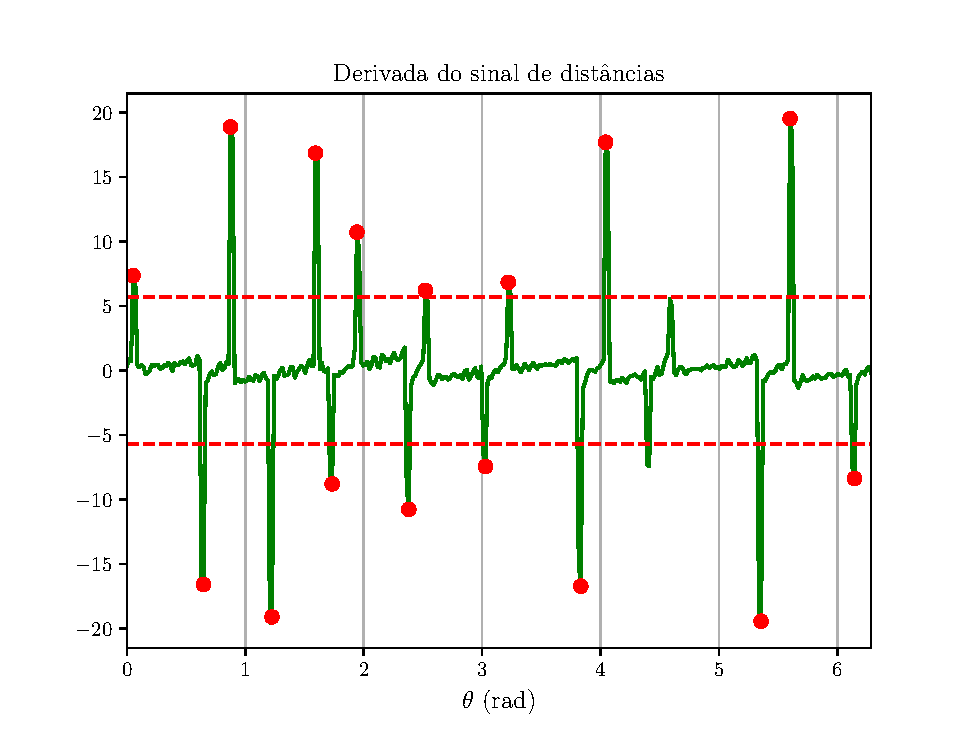
\includegraphics[width=.6\textwidth]{figs/signal_derivative.tex}
\end{figure}


\section{Mapa em grade}
\section{Exploração Autônoma}
